\documentclass{standalone}
\usepackage{tikz}
\usetikzlibrary{patterns}
\usetikzlibrary{positioning}
\usetikzlibrary{patterns, positioning}
\usetikzlibrary{shapes.misc}
\usepackage[outline]{contour}
\contourlength{1.5pt} 
\usetikzlibrary{calc}
        \usepackage{relsize}
        \tikzset{fontscale/.style = {font=\relsize{#1}}}

\begin{document}
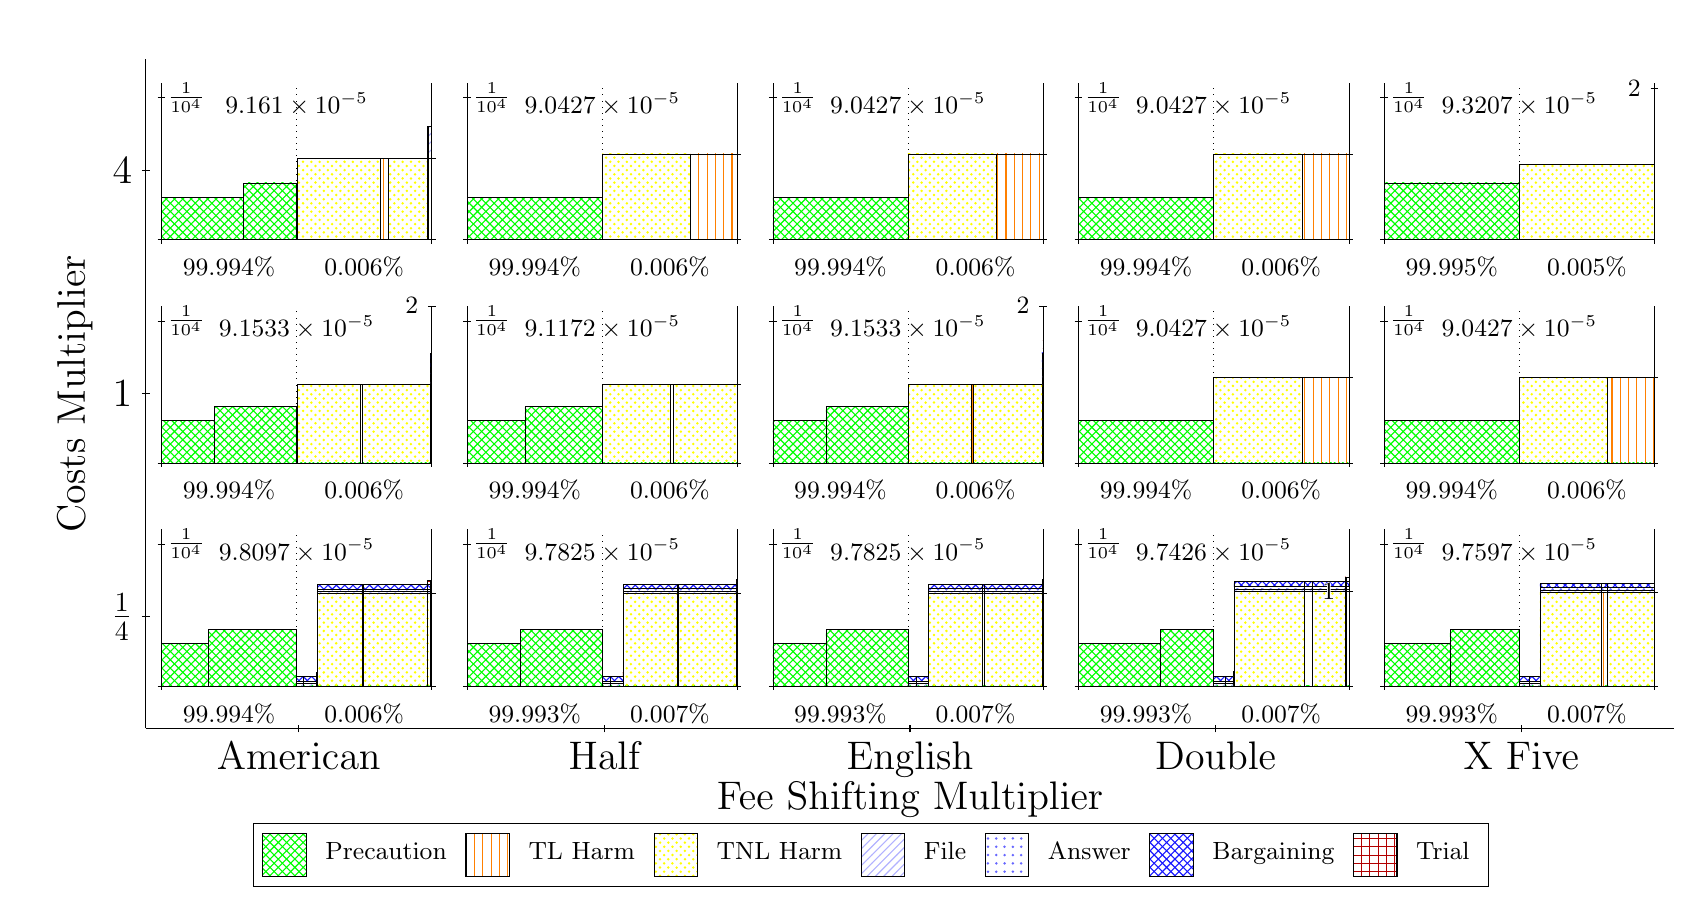
\begin{tikzpicture}
\clip(-0.5,-1.1) rectangle +(20.91,11);
\draw[black] (1,1) -- (1,9.5);
\node[rotate=90, fontscale=2, anchor=center] at (0.1, 5.25) {Costs Multiplier};
\draw[black] (0.95,2.4167) -- (1.05,2.4167);
\node[fontscale=2, anchor=east] at (0.95, 2.4167) {$\frac{1}{4}$};
\draw[black] (0.95,5.25) -- (1.05,5.25);
\node[fontscale=2, anchor=east] at (0.95, 5.25) {1};
\draw[black] (0.95,8.0833) -- (1.05,8.0833);
\node[fontscale=2, anchor=east] at (0.95, 8.0833) {4};

\draw[black] (1,1) -- (20.41,1);
\node[fontscale=2, anchor=center] at (10.705, 0.1) {Fee Shifting Multiplier};
\draw[black] (2.941,0.95) -- (2.941,1.05);
\node[fontscale=2, anchor=north] at (2.941, 0.95) {American};
\draw[black] (6.823,0.95) -- (6.823,1.05);
\node[fontscale=2, anchor=north] at (6.823, 0.95) {Half};
\draw[black] (10.705,0.95) -- (10.705,1.05);
\node[fontscale=2, anchor=north] at (10.705, 0.95) {English};
\draw[black] (14.587,0.95) -- (14.587,1.05);
\node[fontscale=2, anchor=north] at (14.587, 0.95) {Double};
\draw[black] (18.469,0.95) -- (18.469,1.05);
\node[fontscale=2, anchor=north] at (18.469, 0.95) {X Five};


\draw[pattern=crosshatch, pattern color=green,draw=black,very thin] (1.2,1.54) rectangle (1.7938,2.0809);
\draw[pattern=crosshatch, pattern color=green,draw=black,very thin] (1.7938,1.54) rectangle (2.916,2.2612);
\draw[pattern=crosshatch, pattern color=green,draw=black,very thin] (2.916,1.54) rectangle (2.9984,1.54);
\draw[pattern=north east lines, pattern color=blue!30,draw=black,very thin] (2.916,1.54) rectangle (2.9984,1.5693);
\draw[pattern=dots,  pattern color=blue!60,draw=black,very thin] (2.916,1.5693) rectangle (2.9984,1.5986);
\draw[pattern=crosshatch,      pattern color=blue!90,draw=black,very thin] (2.916,1.5986) rectangle (2.9984,1.6571);
\draw[pattern=crosshatch, pattern color=green,draw=black,very thin] (2.9984,1.54) rectangle (3.1711,1.54);
\draw[pattern=north east lines, pattern color=blue!30,draw=black,very thin] (2.9984,1.54) rectangle (3.1711,1.5693);
\draw[pattern=dots,  pattern color=blue!60,draw=black,very thin] (2.9984,1.5693) rectangle (3.1711,1.5986);
\draw[pattern=crosshatch,      pattern color=blue!90,draw=black,very thin] (2.9984,1.5986) rectangle (3.1711,1.6572);
\draw[pattern=crosshatch, pattern color=green,draw=black,very thin] (3.1711,1.54) rectangle (3.1802,1.54);
\draw[pattern=north east lines, pattern color=blue!30,draw=black,very thin] (3.1711,1.54) rectangle (3.1802,1.5693);
\draw[pattern=dots,  pattern color=blue!60,draw=black,very thin] (3.1711,1.5693) rectangle (3.1802,1.5986);
\draw[pattern=crosshatch,      pattern color=blue!90,draw=black,very thin] (3.1711,1.5986) rectangle (3.1802,1.6571);
\draw[pattern=grid,            pattern color=red!70!black,draw=black,very thin] (3.1711,1.6571) rectangle (3.1802,1.7157);
\draw[pattern=crosshatch, pattern color=green,draw=black,very thin] (3.1802,1.54) rectangle (3.7555,1.54);
\draw[pattern=crosshatch dots, pattern color=yellow,draw=black,very thin] (3.1802,1.54) rectangle (3.7555,2.7111);
\draw[pattern=north east lines, pattern color=blue!30,draw=black,very thin] (3.1802,2.7111) rectangle (3.7555,2.7404);
\draw[pattern=dots,  pattern color=blue!60,draw=black,very thin] (3.1802,2.7404) rectangle (3.7555,2.7696);
\draw[pattern=crosshatch,      pattern color=blue!90,draw=black,very thin] (3.1802,2.7696) rectangle (3.7555,2.8282);
\draw[pattern=crosshatch, pattern color=green,draw=black,very thin] (3.7555,1.54) rectangle (3.7609,1.54);
\draw[pattern=vertical lines, pattern color=orange,draw=black,very thin] (3.7555,1.54) rectangle (3.7609,2.7111);
\draw[pattern=north east lines, pattern color=blue!30,draw=black,very thin] (3.7555,2.7111) rectangle (3.7609,2.7404);
\draw[pattern=dots,  pattern color=blue!60,draw=black,very thin] (3.7555,2.7404) rectangle (3.7609,2.7696);
\draw[pattern=crosshatch,      pattern color=blue!90,draw=black,very thin] (3.7555,2.7696) rectangle (3.7609,2.8282);
\draw[pattern=crosshatch, pattern color=green,draw=black,very thin] (3.7609,1.54) rectangle (4.5771,1.54);
\draw[pattern=crosshatch dots, pattern color=yellow,draw=black,very thin] (3.7609,1.54) rectangle (4.5771,2.7111);
\draw[pattern=north east lines, pattern color=blue!30,draw=black,very thin] (3.7609,2.7111) rectangle (4.5771,2.7404);
\draw[pattern=dots,  pattern color=blue!60,draw=black,very thin] (3.7609,2.7404) rectangle (4.5771,2.7697);
\draw[pattern=crosshatch,      pattern color=blue!90,draw=black,very thin] (3.7609,2.7697) rectangle (4.5771,2.8282);
\draw[pattern=crosshatch, pattern color=green,draw=black,very thin] (4.5771,1.54) rectangle (4.6183,1.54);
\draw[pattern=crosshatch dots, pattern color=yellow,draw=black,very thin] (4.5771,1.54) rectangle (4.6183,2.7111);
\draw[pattern=north east lines, pattern color=blue!30,draw=black,very thin] (4.5771,2.7111) rectangle (4.6183,2.7404);
\draw[pattern=dots,  pattern color=blue!60,draw=black,very thin] (4.5771,2.7404) rectangle (4.6183,2.7696);
\draw[pattern=crosshatch,      pattern color=blue!90,draw=black,very thin] (4.5771,2.7696) rectangle (4.6183,2.8282);
\draw[pattern=grid,            pattern color=red!70!black,draw=black,very thin] (4.5771,2.8282) rectangle (4.6183,2.8868);
\draw[pattern=crosshatch, pattern color=green,draw=black,very thin] (4.6183,1.54) rectangle (4.632,1.54);
\draw[pattern=vertical lines, pattern color=orange,draw=black,very thin] (4.6183,1.54) rectangle (4.632,2.7111);
\draw[pattern=north east lines, pattern color=blue!30,draw=black,very thin] (4.6183,2.7111) rectangle (4.632,2.7404);
\draw[pattern=dots,  pattern color=blue!60,draw=black,very thin] (4.6183,2.7404) rectangle (4.632,2.7696);
\draw[pattern=crosshatch,      pattern color=blue!90,draw=black,very thin] (4.6183,2.7696) rectangle (4.632,2.8282);
\draw[pattern=grid,            pattern color=red!70!black,draw=black,very thin] (4.6183,2.8282) rectangle (4.632,2.8868);
\node[font=\small,text=black,anchor=north] at (2.916, 3.5333) {$9.8097\times 10^{-5}$};
\draw[black,very thin] (1.2,1.54) -- (1.2,3.5333);
\draw[black,very thin] (1.15,1.54) -- (1.25,1.54);
\node[font=\small,text=black, anchor=west] at (1.15, 1.54) {};
\draw[black,very thin] (1.15,3.3431) -- (1.25,3.3431);
\node[font=\small,text=black, anchor=west] at (1.15, 3.3431) {$\frac{1}{10^{4}}$};

\draw[black,dotted,very thin] (2.916,1.5998) -- (2.916,3.4735);
\draw[black,very thin] (4.632,1.54) -- (4.632,3.5333);
\draw[black,very thin] (4.582,1.54) -- (4.682,1.54);
\node[font=\small,text=black, anchor=east] at (4.582, 1.54) {\contour{white}{}};
\draw[black,very thin] (4.582,2.7111) -- (4.682,2.7111);
\node[font=\small,text=black, anchor=east] at (4.582, 2.7111) {\contour{white}{}};

\draw[black,very thin] (1.2,1.54) -- (4.632,1.54);
\draw[black,very thin] (1.2,1.49) -- (1.2,1.59);
\node[font=\small,text=black, anchor=north] at (1.2, 1.49) {};
\draw[black,very thin] (4.632,1.49) -- (4.632,1.59);
\node[font=\small,text=black, anchor=north] at (4.632, 1.49) {};

\node[font=\small,text=black,anchor=south] at (2.058, 0.94) {99.994\%};
\node[font=\small,text=black,anchor=south] at (3.774, 0.94) {0.006\%};

\draw[pattern=crosshatch, pattern color=green,draw=black,very thin] (5.082,1.54) rectangle (5.7545,2.0809);
\draw[pattern=crosshatch, pattern color=green,draw=black,very thin] (5.7545,1.54) rectangle (6.798,2.2612);
\draw[pattern=crosshatch, pattern color=green,draw=black,very thin] (6.798,1.54) rectangle (6.8987,1.54);
\draw[pattern=north east lines, pattern color=blue!30,draw=black,very thin] (6.798,1.54) rectangle (6.8987,1.5694);
\draw[pattern=dots,  pattern color=blue!60,draw=black,very thin] (6.798,1.5694) rectangle (6.8987,1.5988);
\draw[pattern=crosshatch,      pattern color=blue!90,draw=black,very thin] (6.798,1.5988) rectangle (6.8987,1.6576);
\draw[pattern=crosshatch, pattern color=green,draw=black,very thin] (6.8987,1.54) rectangle (7.0587,1.54);
\draw[pattern=north east lines, pattern color=blue!30,draw=black,very thin] (6.8987,1.54) rectangle (7.0587,1.5694);
\draw[pattern=dots,  pattern color=blue!60,draw=black,very thin] (6.8987,1.5694) rectangle (7.0587,1.5988);
\draw[pattern=crosshatch,      pattern color=blue!90,draw=black,very thin] (6.8987,1.5988) rectangle (7.0587,1.6576);
\draw[pattern=crosshatch, pattern color=green,draw=black,very thin] (7.0587,1.54) rectangle (7.0612,1.54);
\draw[pattern=north east lines, pattern color=blue!30,draw=black,very thin] (7.0587,1.54) rectangle (7.0612,1.5694);
\draw[pattern=dots,  pattern color=blue!60,draw=black,very thin] (7.0587,1.5694) rectangle (7.0612,1.5988);
\draw[pattern=crosshatch,      pattern color=blue!90,draw=black,very thin] (7.0587,1.5988) rectangle (7.0612,1.6576);
\draw[pattern=grid,            pattern color=red!70!black,draw=black,very thin] (7.0587,1.6576) rectangle (7.0612,1.7164);
\draw[pattern=crosshatch, pattern color=green,draw=black,very thin] (7.0612,1.54) rectangle (7.7449,1.54);
\draw[pattern=crosshatch dots, pattern color=yellow,draw=black,very thin] (7.0612,1.54) rectangle (7.7449,2.7156);
\draw[pattern=north east lines, pattern color=blue!30,draw=black,very thin] (7.0612,2.7156) rectangle (7.7449,2.745);
\draw[pattern=dots,  pattern color=blue!60,draw=black,very thin] (7.0612,2.745) rectangle (7.7449,2.7744);
\draw[pattern=crosshatch,      pattern color=blue!90,draw=black,very thin] (7.0612,2.7744) rectangle (7.7449,2.8332);
\draw[pattern=crosshatch, pattern color=green,draw=black,very thin] (7.7449,1.54) rectangle (7.7615,1.54);
\draw[pattern=vertical lines, pattern color=orange,draw=black,very thin] (7.7449,1.54) rectangle (7.7615,2.7156);
\draw[pattern=north east lines, pattern color=blue!30,draw=black,very thin] (7.7449,2.7156) rectangle (7.7615,2.745);
\draw[pattern=dots,  pattern color=blue!60,draw=black,very thin] (7.7449,2.745) rectangle (7.7615,2.7744);
\draw[pattern=crosshatch,      pattern color=blue!90,draw=black,very thin] (7.7449,2.7744) rectangle (7.7615,2.8332);
\draw[pattern=crosshatch, pattern color=green,draw=black,very thin] (7.7615,1.54) rectangle (8.5,1.54);
\draw[pattern=crosshatch dots, pattern color=yellow,draw=black,very thin] (7.7615,1.54) rectangle (8.5,2.7156);
\draw[pattern=north east lines, pattern color=blue!30,draw=black,very thin] (7.7615,2.7156) rectangle (8.5,2.745);
\draw[pattern=dots,  pattern color=blue!60,draw=black,very thin] (7.7615,2.745) rectangle (8.5,2.7744);
\draw[pattern=crosshatch,      pattern color=blue!90,draw=black,very thin] (7.7615,2.7744) rectangle (8.5,2.8332);
\draw[pattern=crosshatch, pattern color=green,draw=black,very thin] (8.5,1.54) rectangle (8.5069,1.54);
\draw[pattern=crosshatch dots, pattern color=yellow,draw=black,very thin] (8.5,1.54) rectangle (8.5069,2.7156);
\draw[pattern=north east lines, pattern color=blue!30,draw=black,very thin] (8.5,2.7156) rectangle (8.5069,2.745);
\draw[pattern=dots,  pattern color=blue!60,draw=black,very thin] (8.5,2.745) rectangle (8.5069,2.7744);
\draw[pattern=crosshatch,      pattern color=blue!90,draw=black,very thin] (8.5,2.7744) rectangle (8.5069,2.8332);
\draw[pattern=grid,            pattern color=red!70!black,draw=black,very thin] (8.5,2.8332) rectangle (8.5069,2.892);
\draw[pattern=crosshatch, pattern color=green,draw=black,very thin] (8.5069,1.54) rectangle (8.514,1.54);
\draw[pattern=vertical lines, pattern color=orange,draw=black,very thin] (8.5069,1.54) rectangle (8.514,2.7156);
\draw[pattern=north east lines, pattern color=blue!30,draw=black,very thin] (8.5069,2.7156) rectangle (8.514,2.745);
\draw[pattern=dots,  pattern color=blue!60,draw=black,very thin] (8.5069,2.745) rectangle (8.514,2.7744);
\draw[pattern=crosshatch,      pattern color=blue!90,draw=black,very thin] (8.5069,2.7744) rectangle (8.514,2.8332);
\draw[pattern=grid,            pattern color=red!70!black,draw=black,very thin] (8.5069,2.8332) rectangle (8.514,2.892);
\node[font=\small,text=black,anchor=north] at (6.798, 3.5333) {$9.7825\times 10^{-5}$};
\draw[black,very thin] (5.082,1.54) -- (5.082,3.5333);
\draw[black,very thin] (5.032,1.54) -- (5.132,1.54);
\node[font=\small,text=black, anchor=west] at (5.032, 1.54) {};
\draw[black,very thin] (5.032,3.3431) -- (5.132,3.3431);
\node[font=\small,text=black, anchor=west] at (5.032, 3.3431) {$\frac{1}{10^{4}}$};

\draw[black,dotted,very thin] (6.798,1.5998) -- (6.798,3.4735);
\draw[black,very thin] (8.514,1.54) -- (8.514,3.5333);
\draw[black,very thin] (8.464,1.54) -- (8.564,1.54);
\node[font=\small,text=black, anchor=east] at (8.464, 1.54) {\contour{white}{}};
\draw[black,very thin] (8.464,2.7156) -- (8.564,2.7156);
\node[font=\small,text=black, anchor=east] at (8.464, 2.7156) {\contour{white}{}};

\draw[black,very thin] (5.082,1.54) -- (8.514,1.54);
\draw[black,very thin] (5.082,1.49) -- (5.082,1.59);
\node[font=\small,text=black, anchor=north] at (5.082, 1.49) {};
\draw[black,very thin] (8.514,1.49) -- (8.514,1.59);
\node[font=\small,text=black, anchor=north] at (8.514, 1.49) {};

\node[font=\small,text=black,anchor=south] at (5.94, 0.94) {99.993\%};
\node[font=\small,text=black,anchor=south] at (7.656, 0.94) {0.007\%};

\draw[pattern=crosshatch, pattern color=green,draw=black,very thin] (8.964,1.54) rectangle (9.6365,2.0809);
\draw[pattern=crosshatch, pattern color=green,draw=black,very thin] (9.6365,1.54) rectangle (10.68,2.2612);
\draw[pattern=crosshatch, pattern color=green,draw=black,very thin] (10.68,1.54) rectangle (10.781,1.54);
\draw[pattern=north east lines, pattern color=blue!30,draw=black,very thin] (10.68,1.54) rectangle (10.781,1.5694);
\draw[pattern=dots,  pattern color=blue!60,draw=black,very thin] (10.68,1.5694) rectangle (10.781,1.5988);
\draw[pattern=crosshatch,      pattern color=blue!90,draw=black,very thin] (10.68,1.5988) rectangle (10.781,1.6576);
\draw[pattern=crosshatch, pattern color=green,draw=black,very thin] (10.781,1.54) rectangle (10.941,1.54);
\draw[pattern=north east lines, pattern color=blue!30,draw=black,very thin] (10.781,1.54) rectangle (10.941,1.5694);
\draw[pattern=dots,  pattern color=blue!60,draw=black,very thin] (10.781,1.5694) rectangle (10.941,1.5988);
\draw[pattern=crosshatch,      pattern color=blue!90,draw=black,very thin] (10.781,1.5988) rectangle (10.941,1.6576);
\draw[pattern=crosshatch, pattern color=green,draw=black,very thin] (10.941,1.54) rectangle (10.943,1.54);
\draw[pattern=north east lines, pattern color=blue!30,draw=black,very thin] (10.941,1.54) rectangle (10.943,1.5694);
\draw[pattern=dots,  pattern color=blue!60,draw=black,very thin] (10.941,1.5694) rectangle (10.943,1.5988);
\draw[pattern=crosshatch,      pattern color=blue!90,draw=black,very thin] (10.941,1.5988) rectangle (10.943,1.6576);
\draw[pattern=grid,            pattern color=red!70!black,draw=black,very thin] (10.941,1.6576) rectangle (10.943,1.7164);
\draw[pattern=crosshatch, pattern color=green,draw=black,very thin] (10.943,1.54) rectangle (11.627,1.54);
\draw[pattern=crosshatch dots, pattern color=yellow,draw=black,very thin] (10.943,1.54) rectangle (11.627,2.7156);
\draw[pattern=north east lines, pattern color=blue!30,draw=black,very thin] (10.943,2.7156) rectangle (11.627,2.745);
\draw[pattern=dots,  pattern color=blue!60,draw=black,very thin] (10.943,2.745) rectangle (11.627,2.7744);
\draw[pattern=crosshatch,      pattern color=blue!90,draw=black,very thin] (10.943,2.7744) rectangle (11.627,2.8332);
\draw[pattern=crosshatch, pattern color=green,draw=black,very thin] (11.627,1.54) rectangle (11.643,1.54);
\draw[pattern=vertical lines, pattern color=orange,draw=black,very thin] (11.627,1.54) rectangle (11.643,2.7156);
\draw[pattern=north east lines, pattern color=blue!30,draw=black,very thin] (11.627,2.7156) rectangle (11.643,2.745);
\draw[pattern=dots,  pattern color=blue!60,draw=black,very thin] (11.627,2.745) rectangle (11.643,2.7744);
\draw[pattern=crosshatch,      pattern color=blue!90,draw=black,very thin] (11.627,2.7744) rectangle (11.643,2.8332);
\draw[pattern=crosshatch, pattern color=green,draw=black,very thin] (11.643,1.54) rectangle (12.382,1.54);
\draw[pattern=crosshatch dots, pattern color=yellow,draw=black,very thin] (11.643,1.54) rectangle (12.382,2.7156);
\draw[pattern=north east lines, pattern color=blue!30,draw=black,very thin] (11.643,2.7156) rectangle (12.382,2.745);
\draw[pattern=dots,  pattern color=blue!60,draw=black,very thin] (11.643,2.745) rectangle (12.382,2.7744);
\draw[pattern=crosshatch,      pattern color=blue!90,draw=black,very thin] (11.643,2.7744) rectangle (12.382,2.8332);
\draw[pattern=crosshatch, pattern color=green,draw=black,very thin] (12.382,1.54) rectangle (12.389,1.54);
\draw[pattern=crosshatch dots, pattern color=yellow,draw=black,very thin] (12.382,1.54) rectangle (12.389,2.7156);
\draw[pattern=north east lines, pattern color=blue!30,draw=black,very thin] (12.382,2.7156) rectangle (12.389,2.745);
\draw[pattern=dots,  pattern color=blue!60,draw=black,very thin] (12.382,2.745) rectangle (12.389,2.7744);
\draw[pattern=crosshatch,      pattern color=blue!90,draw=black,very thin] (12.382,2.7744) rectangle (12.389,2.8332);
\draw[pattern=grid,            pattern color=red!70!black,draw=black,very thin] (12.382,2.8332) rectangle (12.389,2.892);
\draw[pattern=crosshatch, pattern color=green,draw=black,very thin] (12.389,1.54) rectangle (12.396,1.54);
\draw[pattern=vertical lines, pattern color=orange,draw=black,very thin] (12.389,1.54) rectangle (12.396,2.7156);
\draw[pattern=north east lines, pattern color=blue!30,draw=black,very thin] (12.389,2.7156) rectangle (12.396,2.745);
\draw[pattern=dots,  pattern color=blue!60,draw=black,very thin] (12.389,2.745) rectangle (12.396,2.7744);
\draw[pattern=crosshatch,      pattern color=blue!90,draw=black,very thin] (12.389,2.7744) rectangle (12.396,2.8332);
\draw[pattern=grid,            pattern color=red!70!black,draw=black,very thin] (12.389,2.8332) rectangle (12.396,2.892);
\node[font=\small,text=black,anchor=north] at (10.68, 3.5333) {$9.7825\times 10^{-5}$};
\draw[black,very thin] (8.964,1.54) -- (8.964,3.5333);
\draw[black,very thin] (8.914,1.54) -- (9.014,1.54);
\node[font=\small,text=black, anchor=west] at (8.914, 1.54) {};
\draw[black,very thin] (8.914,3.3431) -- (9.014,3.3431);
\node[font=\small,text=black, anchor=west] at (8.914, 3.3431) {$\frac{1}{10^{4}}$};

\draw[black,dotted,very thin] (10.68,1.5998) -- (10.68,3.4735);
\draw[black,very thin] (12.396,1.54) -- (12.396,3.5333);
\draw[black,very thin] (12.346,1.54) -- (12.446,1.54);
\node[font=\small,text=black, anchor=east] at (12.346, 1.54) {\contour{white}{}};
\draw[black,very thin] (12.346,2.7156) -- (12.446,2.7156);
\node[font=\small,text=black, anchor=east] at (12.346, 2.7156) {\contour{white}{}};

\draw[black,very thin] (8.964,1.54) -- (12.396,1.54);
\draw[black,very thin] (8.964,1.49) -- (8.964,1.59);
\node[font=\small,text=black, anchor=north] at (8.964, 1.49) {};
\draw[black,very thin] (12.396,1.49) -- (12.396,1.59);
\node[font=\small,text=black, anchor=north] at (12.396, 1.49) {};

\node[font=\small,text=black,anchor=south] at (9.822, 0.94) {99.993\%};
\node[font=\small,text=black,anchor=south] at (11.538, 0.94) {0.007\%};

\draw[pattern=crosshatch, pattern color=green,draw=black,very thin] (12.846,1.54) rectangle (13.89,2.0809);
\draw[pattern=crosshatch, pattern color=green,draw=black,very thin] (13.89,1.54) rectangle (14.562,2.2612);
\draw[pattern=crosshatch, pattern color=green,draw=black,very thin] (14.562,1.54) rectangle (14.711,1.54);
\draw[pattern=north east lines, pattern color=blue!30,draw=black,very thin] (14.562,1.54) rectangle (14.711,1.5701);
\draw[pattern=dots,  pattern color=blue!60,draw=black,very thin] (14.562,1.5701) rectangle (14.711,1.6002);
\draw[pattern=crosshatch,      pattern color=blue!90,draw=black,very thin] (14.562,1.6002) rectangle (14.711,1.6604);
\draw[pattern=crosshatch, pattern color=green,draw=black,very thin] (14.711,1.54) rectangle (14.812,1.54);
\draw[pattern=north east lines, pattern color=blue!30,draw=black,very thin] (14.711,1.54) rectangle (14.812,1.5701);
\draw[pattern=dots,  pattern color=blue!60,draw=black,very thin] (14.711,1.5701) rectangle (14.812,1.6002);
\draw[pattern=crosshatch,      pattern color=blue!90,draw=black,very thin] (14.711,1.6002) rectangle (14.812,1.6604);
\draw[pattern=crosshatch, pattern color=green,draw=black,very thin] (14.812,1.54) rectangle (14.819,1.54);
\draw[pattern=north east lines, pattern color=blue!30,draw=black,very thin] (14.812,1.54) rectangle (14.819,1.5701);
\draw[pattern=dots,  pattern color=blue!60,draw=black,very thin] (14.812,1.5701) rectangle (14.819,1.6002);
\draw[pattern=crosshatch,      pattern color=blue!90,draw=black,very thin] (14.812,1.6002) rectangle (14.819,1.6604);
\draw[pattern=grid,            pattern color=red!70!black,draw=black,very thin] (14.812,1.6604) rectangle (14.819,1.7206);
\draw[pattern=crosshatch, pattern color=green,draw=black,very thin] (14.819,1.54) rectangle (15.719,1.54);
\draw[pattern=crosshatch dots, pattern color=yellow,draw=black,very thin] (14.819,1.54) rectangle (15.719,2.7435);
\draw[pattern=north east lines, pattern color=blue!30,draw=black,very thin] (14.819,2.7435) rectangle (15.719,2.7736);
\draw[pattern=dots,  pattern color=blue!60,draw=black,very thin] (14.819,2.7736) rectangle (15.719,2.8037);
\draw[pattern=crosshatch,      pattern color=blue!90,draw=black,very thin] (14.819,2.8037) rectangle (15.719,2.8639);
\draw[pattern=crosshatch, pattern color=green,draw=black,very thin] (15.719,1.54) rectangle (15.811,1.54);
\draw[pattern=vertical lines, pattern color=orange,draw=black,very thin] (15.719,1.54) rectangle (15.811,2.7435);
\draw[pattern=north east lines, pattern color=blue!30,draw=black,very thin] (15.719,2.7435) rectangle (15.811,2.7736);
\draw[pattern=dots,  pattern color=blue!60,draw=black,very thin] (15.719,2.7736) rectangle (15.811,2.8037);
\draw[pattern=crosshatch,      pattern color=blue!90,draw=black,very thin] (15.719,2.8037) rectangle (15.811,2.8639);
\draw[pattern=crosshatch, pattern color=green,draw=black,very thin] (15.811,1.54) rectangle (16.238,1.54);
\draw[pattern=crosshatch dots, pattern color=yellow,draw=black,very thin] (15.811,1.54) rectangle (16.238,2.7435);
\draw[pattern=north east lines, pattern color=blue!30,draw=black,very thin] (15.811,2.7435) rectangle (16.238,2.7736);
\draw[pattern=dots,  pattern color=blue!60,draw=black,very thin] (15.811,2.7736) rectangle (16.238,2.8037);
\draw[pattern=crosshatch,      pattern color=blue!90,draw=black,very thin] (15.811,2.8037) rectangle (16.238,2.8639);
\draw[pattern=crosshatch, pattern color=green,draw=black,very thin] (16.238,1.54) rectangle (16.248,1.54);
\draw[pattern=crosshatch dots, pattern color=yellow,draw=black,very thin] (16.238,1.54) rectangle (16.248,2.7435);
\draw[pattern=north east lines, pattern color=blue!30,draw=black,very thin] (16.238,2.7435) rectangle (16.248,2.7736);
\draw[pattern=dots,  pattern color=blue!60,draw=black,very thin] (16.238,2.7736) rectangle (16.248,2.8037);
\draw[pattern=crosshatch,      pattern color=blue!90,draw=black,very thin] (16.238,2.8037) rectangle (16.248,2.8639);
\draw[pattern=grid,            pattern color=red!70!black,draw=black,very thin] (16.238,2.8639) rectangle (16.248,2.924);
\draw[pattern=crosshatch, pattern color=green,draw=black,very thin] (16.248,1.54) rectangle (16.278,1.54);
\draw[pattern=vertical lines, pattern color=orange,draw=black,very thin] (16.248,1.54) rectangle (16.278,2.7435);
\draw[pattern=north east lines, pattern color=blue!30,draw=black,very thin] (16.248,2.7435) rectangle (16.278,2.7736);
\draw[pattern=dots,  pattern color=blue!60,draw=black,very thin] (16.248,2.7736) rectangle (16.278,2.8037);
\draw[pattern=crosshatch,      pattern color=blue!90,draw=black,very thin] (16.248,2.8037) rectangle (16.278,2.8639);
\draw[pattern=grid,            pattern color=red!70!black,draw=black,very thin] (16.248,2.8639) rectangle (16.278,2.924);
\node[font=\small,text=black,anchor=north] at (14.562, 3.5333) {$9.7426\times 10^{-5}$};
\draw[black,very thin] (12.846,1.54) -- (12.846,3.5333);
\draw[black,very thin] (12.796,1.54) -- (12.896,1.54);
\node[font=\small,text=black, anchor=west] at (12.796, 1.54) {};
\draw[black,very thin] (12.796,3.3431) -- (12.896,3.3431);
\node[font=\small,text=black, anchor=west] at (12.796, 3.3431) {$\frac{1}{10^{4}}$};

\draw[black,dotted,very thin] (14.562,1.5998) -- (14.562,3.4735);
\draw[black,very thin] (16.278,1.54) -- (16.278,3.5333);
\draw[black,very thin] (16.228,1.54) -- (16.328,1.54);
\node[font=\small,text=black, anchor=east] at (16.228, 1.54) {\contour{white}{}};
\draw[black,very thin] (16.228,2.7435) -- (16.328,2.7435);
\node[font=\small,text=black, anchor=east] at (16.228, 2.7435) {\contour{white}{1}};

\draw[black,very thin] (12.846,1.54) -- (16.278,1.54);
\draw[black,very thin] (12.846,1.49) -- (12.846,1.59);
\node[font=\small,text=black, anchor=north] at (12.846, 1.49) {};
\draw[black,very thin] (16.278,1.49) -- (16.278,1.59);
\node[font=\small,text=black, anchor=north] at (16.278, 1.49) {};

\node[font=\small,text=black,anchor=south] at (13.704, 0.94) {99.993\%};
\node[font=\small,text=black,anchor=south] at (15.42, 0.94) {0.007\%};

\draw[pattern=crosshatch, pattern color=green,draw=black,very thin] (16.728,1.54) rectangle (17.561,2.0809);
\draw[pattern=crosshatch, pattern color=green,draw=black,very thin] (17.561,1.54) rectangle (18.444,2.2612);
\draw[pattern=crosshatch, pattern color=green,draw=black,very thin] (18.444,1.54) rectangle (18.57,1.54);
\draw[pattern=north east lines, pattern color=blue!30,draw=black,very thin] (18.444,1.54) rectangle (18.57,1.5697);
\draw[pattern=dots,  pattern color=blue!60,draw=black,very thin] (18.444,1.5697) rectangle (18.57,1.5994);
\draw[pattern=crosshatch,      pattern color=blue!90,draw=black,very thin] (18.444,1.5994) rectangle (18.57,1.6588);
\draw[pattern=crosshatch, pattern color=green,draw=black,very thin] (18.57,1.54) rectangle (18.704,1.54);
\draw[pattern=north east lines, pattern color=blue!30,draw=black,very thin] (18.57,1.54) rectangle (18.704,1.5697);
\draw[pattern=dots,  pattern color=blue!60,draw=black,very thin] (18.57,1.5697) rectangle (18.704,1.5994);
\draw[pattern=crosshatch,      pattern color=blue!90,draw=black,very thin] (18.57,1.5994) rectangle (18.704,1.6588);
\draw[pattern=crosshatch, pattern color=green,draw=black,very thin] (18.704,1.54) rectangle (19.489,1.54);
\draw[pattern=crosshatch dots, pattern color=yellow,draw=black,very thin] (18.704,1.54) rectangle (19.489,2.7274);
\draw[pattern=north east lines, pattern color=blue!30,draw=black,very thin] (18.704,2.7274) rectangle (19.489,2.7571);
\draw[pattern=dots,  pattern color=blue!60,draw=black,very thin] (18.704,2.7571) rectangle (19.489,2.7868);
\draw[pattern=crosshatch,      pattern color=blue!90,draw=black,very thin] (18.704,2.7868) rectangle (19.489,2.8461);
\draw[pattern=crosshatch, pattern color=green,draw=black,very thin] (19.489,1.54) rectangle (19.556,1.54);
\draw[pattern=vertical lines, pattern color=orange,draw=black,very thin] (19.489,1.54) rectangle (19.556,2.7274);
\draw[pattern=north east lines, pattern color=blue!30,draw=black,very thin] (19.489,2.7274) rectangle (19.556,2.7571);
\draw[pattern=dots,  pattern color=blue!60,draw=black,very thin] (19.489,2.7571) rectangle (19.556,2.7868);
\draw[pattern=crosshatch,      pattern color=blue!90,draw=black,very thin] (19.489,2.7868) rectangle (19.556,2.8461);
\draw[pattern=crosshatch, pattern color=green,draw=black,very thin] (19.556,1.54) rectangle (20.158,1.54);
\draw[pattern=crosshatch dots, pattern color=yellow,draw=black,very thin] (19.556,1.54) rectangle (20.158,2.7274);
\draw[pattern=north east lines, pattern color=blue!30,draw=black,very thin] (19.556,2.7274) rectangle (20.158,2.7571);
\draw[pattern=dots,  pattern color=blue!60,draw=black,very thin] (19.556,2.7571) rectangle (20.158,2.7868);
\draw[pattern=crosshatch,      pattern color=blue!90,draw=black,very thin] (19.556,2.7868) rectangle (20.158,2.8461);
\draw[pattern=crosshatch, pattern color=green,draw=black,very thin] (20.158,1.54) rectangle (20.159,1.54);
\draw[pattern=crosshatch dots, pattern color=yellow,draw=black,very thin] (20.158,1.54) rectangle (20.159,2.7274);
\draw[pattern=north east lines, pattern color=blue!30,draw=black,very thin] (20.158,2.7274) rectangle (20.159,2.7571);
\draw[pattern=dots,  pattern color=blue!60,draw=black,very thin] (20.158,2.7571) rectangle (20.159,2.7868);
\draw[pattern=crosshatch,      pattern color=blue!90,draw=black,very thin] (20.158,2.7868) rectangle (20.159,2.8461);
\draw[pattern=grid,            pattern color=red!70!black,draw=black,very thin] (20.158,2.8461) rectangle (20.159,2.9055);
\draw[pattern=crosshatch, pattern color=green,draw=black,very thin] (20.159,1.54) rectangle (20.16,1.54);
\draw[pattern=vertical lines, pattern color=orange,draw=black,very thin] (20.159,1.54) rectangle (20.16,2.7274);
\draw[pattern=north east lines, pattern color=blue!30,draw=black,very thin] (20.159,2.7274) rectangle (20.16,2.7571);
\draw[pattern=dots,  pattern color=blue!60,draw=black,very thin] (20.159,2.7571) rectangle (20.16,2.7868);
\draw[pattern=crosshatch,      pattern color=blue!90,draw=black,very thin] (20.159,2.7868) rectangle (20.16,2.8461);
\draw[pattern=grid,            pattern color=red!70!black,draw=black,very thin] (20.159,2.8461) rectangle (20.16,2.9055);
\node[font=\small,text=black,anchor=north] at (18.444, 3.5333) {$9.7597\times 10^{-5}$};
\draw[black,very thin] (16.728,1.54) -- (16.728,3.5333);
\draw[black,very thin] (16.678,1.54) -- (16.778,1.54);
\node[font=\small,text=black, anchor=west] at (16.678, 1.54) {};
\draw[black,very thin] (16.678,3.3431) -- (16.778,3.3431);
\node[font=\small,text=black, anchor=west] at (16.678, 3.3431) {$\frac{1}{10^{4}}$};

\draw[black,dotted,very thin] (18.444,1.5998) -- (18.444,3.4735);
\draw[black,very thin] (20.16,1.54) -- (20.16,3.5333);
\draw[black,very thin] (20.11,1.54) -- (20.21,1.54);
\node[font=\small,text=black, anchor=east] at (20.11, 1.54) {\contour{white}{}};
\draw[black,very thin] (20.11,2.7274) -- (20.21,2.7274);
\node[font=\small,text=black, anchor=east] at (20.11, 2.7274) {\contour{white}{}};

\draw[black,very thin] (16.728,1.54) -- (20.16,1.54);
\draw[black,very thin] (16.728,1.49) -- (16.728,1.59);
\node[font=\small,text=black, anchor=north] at (16.728, 1.49) {};
\draw[black,very thin] (20.16,1.49) -- (20.16,1.59);
\node[font=\small,text=black, anchor=north] at (20.16, 1.49) {};

\node[font=\small,text=black,anchor=south] at (17.586, 0.94) {99.993\%};
\node[font=\small,text=black,anchor=south] at (19.302, 0.94) {0.007\%};

\draw[pattern=crosshatch, pattern color=green,draw=black,very thin] (1.2,4.3733) rectangle (1.8725,4.9143);
\draw[pattern=crosshatch, pattern color=green,draw=black,very thin] (1.8725,4.3733) rectangle (2.916,5.0946);
\draw[pattern=crosshatch, pattern color=green,draw=black,very thin] (2.916,4.3733) rectangle (2.9185,4.3734);
\draw[pattern=north east lines, pattern color=blue!30,draw=black,very thin] (2.916,4.3734) rectangle (2.9185,4.473);
\draw[pattern=dots,  pattern color=blue!60,draw=black,very thin] (2.916,4.473) rectangle (2.9185,4.5727);
\draw[pattern=crosshatch,      pattern color=blue!90,draw=black,very thin] (2.916,4.5727) rectangle (2.9185,4.772);
\draw[pattern=crosshatch, pattern color=green,draw=black,very thin] (2.9185,4.3733) rectangle (3.7249,4.3734);
\draw[pattern=crosshatch dots, pattern color=yellow,draw=black,very thin] (2.9185,4.3734) rectangle (3.7249,5.37);
\draw[pattern=crosshatch, pattern color=green,draw=black,very thin] (3.7249,4.3733) rectangle (3.7444,4.3734);
\draw[pattern=vertical lines, pattern color=orange,draw=black,very thin] (3.7249,4.3734) rectangle (3.7444,5.37);
\draw[pattern=crosshatch, pattern color=green,draw=black,very thin] (3.7444,4.3733) rectangle (4.6156,4.3734);
\draw[pattern=crosshatch dots, pattern color=yellow,draw=black,very thin] (3.7444,4.3734) rectangle (4.6156,5.37);
\draw[pattern=crosshatch, pattern color=green,draw=black,very thin] (4.6156,4.3733) rectangle (4.6216,4.3734);
\draw[pattern=crosshatch dots, pattern color=yellow,draw=black,very thin] (4.6156,4.3734) rectangle (4.6216,5.37);
\draw[pattern=north east lines, pattern color=blue!30,draw=black,very thin] (4.6156,5.37) rectangle (4.6216,5.4697);
\draw[pattern=dots,  pattern color=blue!60,draw=black,very thin] (4.6156,5.4697) rectangle (4.6216,5.5693);
\draw[pattern=crosshatch,      pattern color=blue!90,draw=black,very thin] (4.6156,5.5693) rectangle (4.6216,5.7687);
\draw[pattern=crosshatch, pattern color=green,draw=black,very thin] (4.6216,4.3733) rectangle (4.6292,4.3734);
\draw[pattern=vertical lines, pattern color=orange,draw=black,very thin] (4.6216,4.3734) rectangle (4.6292,5.37);
\draw[pattern=north east lines, pattern color=blue!30,draw=black,very thin] (4.6216,5.37) rectangle (4.6292,5.4697);
\draw[pattern=dots,  pattern color=blue!60,draw=black,very thin] (4.6216,5.4697) rectangle (4.6292,5.5693);
\draw[pattern=crosshatch,      pattern color=blue!90,draw=black,very thin] (4.6216,5.5693) rectangle (4.6292,5.7687);
\draw[pattern=crosshatch, pattern color=green,draw=black,very thin] (4.6292,4.3733) rectangle (4.6313,4.3734);
\draw[pattern=crosshatch dots, pattern color=yellow,draw=black,very thin] (4.6292,4.3734) rectangle (4.6313,5.37);
\draw[pattern=north east lines, pattern color=blue!30,draw=black,very thin] (4.6292,5.37) rectangle (4.6313,5.4697);
\draw[pattern=dots,  pattern color=blue!60,draw=black,very thin] (4.6292,5.4697) rectangle (4.6313,5.5693);
\draw[pattern=crosshatch,      pattern color=blue!90,draw=black,very thin] (4.6292,5.5693) rectangle (4.6313,5.7687);
\draw[pattern=grid,            pattern color=red!70!black,draw=black,very thin] (4.6292,5.7687) rectangle (4.6313,5.968);
\draw[pattern=crosshatch, pattern color=green,draw=black,very thin] (4.6313,4.3733) rectangle (4.632,4.3734);
\draw[pattern=vertical lines, pattern color=orange,draw=black,very thin] (4.6313,4.3734) rectangle (4.632,5.37);
\draw[pattern=north east lines, pattern color=blue!30,draw=black,very thin] (4.6313,5.37) rectangle (4.632,5.4697);
\draw[pattern=dots,  pattern color=blue!60,draw=black,very thin] (4.6313,5.4697) rectangle (4.632,5.5693);
\draw[pattern=crosshatch,      pattern color=blue!90,draw=black,very thin] (4.6313,5.5693) rectangle (4.632,5.7687);
\draw[pattern=grid,            pattern color=red!70!black,draw=black,very thin] (4.6313,5.7687) rectangle (4.632,5.968);
\node[font=\small,text=black,anchor=north] at (2.916, 6.3667) {$9.1533\times 10^{-5}$};
\draw[black,very thin] (1.2,4.3733) -- (1.2,6.3667);
\draw[black,very thin] (1.15,4.3733) -- (1.25,4.3733);
\node[font=\small,text=black, anchor=west] at (1.15, 4.3733) {};
\draw[black,very thin] (1.15,6.1765) -- (1.25,6.1765);
\node[font=\small,text=black, anchor=west] at (1.15, 6.1765) {$\frac{1}{10^{4}}$};

\draw[black,dotted,very thin] (2.916,4.4331) -- (2.916,6.3069);
\draw[black,very thin] (4.632,4.3733) -- (4.632,6.3667);
\draw[black,very thin] (4.582,6.3666) -- (4.682,6.3666);
\node[font=\small,text=black, anchor=east] at (4.582, 6.3666) {\contour{white}{2}};

\draw[black,very thin] (1.2,4.3733) -- (4.632,4.3733);
\draw[black,very thin] (1.2,4.3233) -- (1.2,4.4233);
\node[font=\small,text=black, anchor=north] at (1.2, 4.3233) {};
\draw[black,very thin] (4.632,4.3233) -- (4.632,4.4233);
\node[font=\small,text=black, anchor=north] at (4.632, 4.3233) {};

\node[font=\small,text=black,anchor=south] at (2.058, 3.7733) {99.994\%};
\node[font=\small,text=black,anchor=south] at (3.774, 3.7733) {0.006\%};

\draw[pattern=crosshatch, pattern color=green,draw=black,very thin] (5.082,4.3733) rectangle (5.8159,4.9143);
\draw[pattern=crosshatch, pattern color=green,draw=black,very thin] (5.8159,4.3733) rectangle (6.798,5.0946);
\draw[pattern=crosshatch, pattern color=green,draw=black,very thin] (6.798,4.3733) rectangle (7.6569,4.3734);
\draw[pattern=crosshatch dots, pattern color=yellow,draw=black,very thin] (6.798,4.3734) rectangle (7.6569,5.3732);
\draw[pattern=crosshatch, pattern color=green,draw=black,very thin] (7.6569,4.3733) rectangle (7.7045,4.3734);
\draw[pattern=vertical lines, pattern color=orange,draw=black,very thin] (7.6569,4.3734) rectangle (7.7045,5.3732);
\draw[pattern=crosshatch, pattern color=green,draw=black,very thin] (7.7045,4.3733) rectangle (8.514,4.3734);
\draw[pattern=crosshatch dots, pattern color=yellow,draw=black,very thin] (7.7045,4.3734) rectangle (8.514,5.3732);
\node[font=\small,text=black,anchor=north] at (6.798, 6.3667) {$9.1172\times 10^{-5}$};
\draw[black,very thin] (5.082,4.3733) -- (5.082,6.3667);
\draw[black,very thin] (5.032,4.3733) -- (5.132,4.3733);
\node[font=\small,text=black, anchor=west] at (5.032, 4.3733) {};
\draw[black,very thin] (5.032,6.1765) -- (5.132,6.1765);
\node[font=\small,text=black, anchor=west] at (5.032, 6.1765) {$\frac{1}{10^{4}}$};

\draw[black,dotted,very thin] (6.798,4.4331) -- (6.798,6.3069);
\draw[black,very thin] (8.514,4.3733) -- (8.514,6.3667);
\draw[black,very thin] (8.464,4.3733) -- (8.564,4.3733);
\node[font=\small,text=black, anchor=east] at (8.464, 4.3733) {\contour{white}{}};
\draw[black,very thin] (8.464,5.3732) -- (8.564,5.3732);
\node[font=\small,text=black, anchor=east] at (8.464, 5.3732) {\contour{white}{}};

\draw[black,very thin] (5.082,4.3733) -- (8.514,4.3733);
\draw[black,very thin] (5.082,4.3233) -- (5.082,4.4233);
\node[font=\small,text=black, anchor=north] at (5.082, 4.3233) {};
\draw[black,very thin] (8.514,4.3233) -- (8.514,4.4233);
\node[font=\small,text=black, anchor=north] at (8.514, 4.3233) {};

\node[font=\small,text=black,anchor=south] at (5.94, 3.7733) {99.994\%};
\node[font=\small,text=black,anchor=south] at (7.656, 3.7733) {0.006\%};

\draw[pattern=crosshatch, pattern color=green,draw=black,very thin] (8.964,4.3733) rectangle (9.6365,4.9143);
\draw[pattern=crosshatch, pattern color=green,draw=black,very thin] (9.6365,4.3733) rectangle (10.68,5.0946);
\draw[pattern=crosshatch, pattern color=green,draw=black,very thin] (10.68,4.3733) rectangle (10.682,4.3734);
\draw[pattern=north east lines, pattern color=blue!30,draw=black,very thin] (10.68,4.3734) rectangle (10.682,4.473);
\draw[pattern=dots,  pattern color=blue!60,draw=black,very thin] (10.68,4.473) rectangle (10.682,4.5727);
\draw[pattern=crosshatch,      pattern color=blue!90,draw=black,very thin] (10.68,4.5727) rectangle (10.682,4.772);
\draw[pattern=crosshatch, pattern color=green,draw=black,very thin] (10.682,4.3733) rectangle (11.489,4.3734);
\draw[pattern=crosshatch dots, pattern color=yellow,draw=black,very thin] (10.682,4.3734) rectangle (11.489,5.37);
\draw[pattern=crosshatch, pattern color=green,draw=black,very thin] (11.489,4.3733) rectangle (11.508,4.3734);
\draw[pattern=vertical lines, pattern color=orange,draw=black,very thin] (11.489,4.3734) rectangle (11.508,5.37);
\draw[pattern=crosshatch, pattern color=green,draw=black,very thin] (11.508,4.3733) rectangle (12.38,4.3734);
\draw[pattern=crosshatch dots, pattern color=yellow,draw=black,very thin] (11.508,4.3734) rectangle (12.38,5.37);
\draw[pattern=crosshatch, pattern color=green,draw=black,very thin] (12.38,4.3733) rectangle (12.386,4.3734);
\draw[pattern=crosshatch dots, pattern color=yellow,draw=black,very thin] (12.38,4.3734) rectangle (12.386,5.37);
\draw[pattern=north east lines, pattern color=blue!30,draw=black,very thin] (12.38,5.37) rectangle (12.386,5.4697);
\draw[pattern=dots,  pattern color=blue!60,draw=black,very thin] (12.38,5.4697) rectangle (12.386,5.5693);
\draw[pattern=crosshatch,      pattern color=blue!90,draw=black,very thin] (12.38,5.5693) rectangle (12.386,5.7687);
\draw[pattern=crosshatch, pattern color=green,draw=black,very thin] (12.386,4.3733) rectangle (12.393,4.3734);
\draw[pattern=vertical lines, pattern color=orange,draw=black,very thin] (12.386,4.3734) rectangle (12.393,5.37);
\draw[pattern=north east lines, pattern color=blue!30,draw=black,very thin] (12.386,5.37) rectangle (12.393,5.4697);
\draw[pattern=dots,  pattern color=blue!60,draw=black,very thin] (12.386,5.4697) rectangle (12.393,5.5693);
\draw[pattern=crosshatch,      pattern color=blue!90,draw=black,very thin] (12.386,5.5693) rectangle (12.393,5.7687);
\draw[pattern=crosshatch, pattern color=green,draw=black,very thin] (12.393,4.3733) rectangle (12.395,4.3734);
\draw[pattern=crosshatch dots, pattern color=yellow,draw=black,very thin] (12.393,4.3734) rectangle (12.395,5.37);
\draw[pattern=north east lines, pattern color=blue!30,draw=black,very thin] (12.393,5.37) rectangle (12.395,5.4697);
\draw[pattern=dots,  pattern color=blue!60,draw=black,very thin] (12.393,5.4697) rectangle (12.395,5.5693);
\draw[pattern=crosshatch,      pattern color=blue!90,draw=black,very thin] (12.393,5.5693) rectangle (12.395,5.7687);
\draw[pattern=grid,            pattern color=red!70!black,draw=black,very thin] (12.393,5.7687) rectangle (12.395,5.968);
\draw[pattern=crosshatch, pattern color=green,draw=black,very thin] (12.395,4.3733) rectangle (12.396,4.3734);
\draw[pattern=vertical lines, pattern color=orange,draw=black,very thin] (12.395,4.3734) rectangle (12.396,5.37);
\draw[pattern=north east lines, pattern color=blue!30,draw=black,very thin] (12.395,5.37) rectangle (12.396,5.4697);
\draw[pattern=dots,  pattern color=blue!60,draw=black,very thin] (12.395,5.4697) rectangle (12.396,5.5693);
\draw[pattern=crosshatch,      pattern color=blue!90,draw=black,very thin] (12.395,5.5693) rectangle (12.396,5.7687);
\draw[pattern=grid,            pattern color=red!70!black,draw=black,very thin] (12.395,5.7687) rectangle (12.396,5.968);
\node[font=\small,text=black,anchor=north] at (10.68, 6.3667) {$9.1533\times 10^{-5}$};
\draw[black,very thin] (8.964,4.3733) -- (8.964,6.3667);
\draw[black,very thin] (8.914,4.3733) -- (9.014,4.3733);
\node[font=\small,text=black, anchor=west] at (8.914, 4.3733) {};
\draw[black,very thin] (8.914,6.1765) -- (9.014,6.1765);
\node[font=\small,text=black, anchor=west] at (8.914, 6.1765) {$\frac{1}{10^{4}}$};

\draw[black,dotted,very thin] (10.68,4.4331) -- (10.68,6.3069);
\draw[black,very thin] (12.396,4.3733) -- (12.396,6.3667);
\draw[black,very thin] (12.346,6.3666) -- (12.446,6.3666);
\node[font=\small,text=black, anchor=east] at (12.346, 6.3666) {\contour{white}{2}};

\draw[black,very thin] (8.964,4.3733) -- (12.396,4.3733);
\draw[black,very thin] (8.964,4.3233) -- (8.964,4.4233);
\node[font=\small,text=black, anchor=north] at (8.964, 4.3233) {};
\draw[black,very thin] (12.396,4.3233) -- (12.396,4.4233);
\node[font=\small,text=black, anchor=north] at (12.396, 4.3233) {};

\node[font=\small,text=black,anchor=south] at (9.822, 3.7733) {99.994\%};
\node[font=\small,text=black,anchor=south] at (11.538, 3.7733) {0.006\%};

\draw[pattern=crosshatch, pattern color=green,draw=black,very thin] (12.846,4.3733) rectangle (14.562,4.9143);
\draw[pattern=crosshatch, pattern color=green,draw=black,very thin] (14.562,4.3733) rectangle (15.685,4.3734);
\draw[pattern=crosshatch dots, pattern color=yellow,draw=black,very thin] (14.562,4.3734) rectangle (15.685,5.463);
\draw[pattern=crosshatch, pattern color=green,draw=black,very thin] (15.685,4.3733) rectangle (16.278,4.3734);
\draw[pattern=vertical lines, pattern color=orange,draw=black,very thin] (15.685,4.3734) rectangle (16.278,5.463);
\node[font=\small,text=black,anchor=north] at (14.562, 6.3667) {$9.0427\times 10^{-5}$};
\draw[black,very thin] (12.846,4.3733) -- (12.846,6.3667);
\draw[black,very thin] (12.796,4.3733) -- (12.896,4.3733);
\node[font=\small,text=black, anchor=west] at (12.796, 4.3733) {};
\draw[black,very thin] (12.796,6.1765) -- (12.896,6.1765);
\node[font=\small,text=black, anchor=west] at (12.796, 6.1765) {$\frac{1}{10^{4}}$};

\draw[black,dotted,very thin] (14.562,4.4331) -- (14.562,6.3069);
\draw[black,very thin] (16.278,4.3733) -- (16.278,6.3667);
\draw[black,very thin] (16.228,4.3733) -- (16.328,4.3733);
\node[font=\small,text=black, anchor=east] at (16.228, 4.3733) {\contour{white}{}};
\draw[black,very thin] (16.228,5.463) -- (16.328,5.463);
\node[font=\small,text=black, anchor=east] at (16.228, 5.463) {\contour{white}{}};

\draw[black,very thin] (12.846,4.3733) -- (16.278,4.3733);
\draw[black,very thin] (12.846,4.3233) -- (12.846,4.4233);
\node[font=\small,text=black, anchor=north] at (12.846, 4.3233) {};
\draw[black,very thin] (16.278,4.3233) -- (16.278,4.4233);
\node[font=\small,text=black, anchor=north] at (16.278, 4.3233) {};

\node[font=\small,text=black,anchor=south] at (13.704, 3.7733) {99.994\%};
\node[font=\small,text=black,anchor=south] at (15.42, 3.7733) {0.006\%};

\draw[pattern=crosshatch, pattern color=green,draw=black,very thin] (16.728,4.3733) rectangle (18.444,4.9143);
\draw[pattern=crosshatch, pattern color=green,draw=black,very thin] (18.444,4.3733) rectangle (19.567,4.3734);
\draw[pattern=crosshatch dots, pattern color=yellow,draw=black,very thin] (18.444,4.3734) rectangle (19.567,5.463);
\draw[pattern=crosshatch, pattern color=green,draw=black,very thin] (19.567,4.3733) rectangle (20.16,4.3734);
\draw[pattern=vertical lines, pattern color=orange,draw=black,very thin] (19.567,4.3734) rectangle (20.16,5.463);
\node[font=\small,text=black,anchor=north] at (18.444, 6.3667) {$9.0427\times 10^{-5}$};
\draw[black,very thin] (16.728,4.3733) -- (16.728,6.3667);
\draw[black,very thin] (16.678,4.3733) -- (16.778,4.3733);
\node[font=\small,text=black, anchor=west] at (16.678, 4.3733) {};
\draw[black,very thin] (16.678,6.1765) -- (16.778,6.1765);
\node[font=\small,text=black, anchor=west] at (16.678, 6.1765) {$\frac{1}{10^{4}}$};

\draw[black,dotted,very thin] (18.444,4.4331) -- (18.444,6.3069);
\draw[black,very thin] (20.16,4.3733) -- (20.16,6.3667);
\draw[black,very thin] (20.11,4.3733) -- (20.21,4.3733);
\node[font=\small,text=black, anchor=east] at (20.11, 4.3733) {\contour{white}{}};
\draw[black,very thin] (20.11,5.463) -- (20.21,5.463);
\node[font=\small,text=black, anchor=east] at (20.11, 5.463) {\contour{white}{}};

\draw[black,very thin] (16.728,4.3733) -- (20.16,4.3733);
\draw[black,very thin] (16.728,4.3233) -- (16.728,4.4233);
\node[font=\small,text=black, anchor=north] at (16.728, 4.3233) {};
\draw[black,very thin] (20.16,4.3233) -- (20.16,4.4233);
\node[font=\small,text=black, anchor=north] at (20.16, 4.3233) {};

\node[font=\small,text=black,anchor=south] at (17.586, 3.7733) {99.994\%};
\node[font=\small,text=black,anchor=south] at (19.302, 3.7733) {0.006\%};

\draw[pattern=crosshatch, pattern color=green,draw=black,very thin] (1.2,7.2067) rectangle (2.2435,7.7476);
\draw[pattern=crosshatch, pattern color=green,draw=black,very thin] (2.2435,7.2067) rectangle (2.916,7.9279);
\draw[pattern=crosshatch, pattern color=green,draw=black,very thin] (2.916,7.2067) rectangle (2.9273,7.2067);
\draw[pattern=north east lines, pattern color=blue!30,draw=black,very thin] (2.916,7.2067) rectangle (2.9273,7.6187);
\draw[pattern=crosshatch, pattern color=green,draw=black,very thin] (2.9273,7.2067) rectangle (3.9757,7.2067);
\draw[pattern=crosshatch dots, pattern color=yellow,draw=black,very thin] (2.9273,7.2067) rectangle (3.9757,8.2366);
\draw[pattern=crosshatch, pattern color=green,draw=black,very thin] (3.9757,7.2067) rectangle (4.0739,7.2067);
\draw[pattern=vertical lines, pattern color=orange,draw=black,very thin] (3.9757,7.2067) rectangle (4.0739,8.2366);
\draw[pattern=crosshatch, pattern color=green,draw=black,very thin] (4.0739,7.2067) rectangle (4.5719,7.2067);
\draw[pattern=crosshatch dots, pattern color=yellow,draw=black,very thin] (4.0739,7.2067) rectangle (4.5719,8.2366);
\draw[pattern=crosshatch, pattern color=green,draw=black,very thin] (4.5719,7.2067) rectangle (4.5869,7.2067);
\draw[pattern=crosshatch dots, pattern color=yellow,draw=black,very thin] (4.5719,7.2067) rectangle (4.5869,8.2366);
\draw[pattern=north east lines, pattern color=blue!30,draw=black,very thin] (4.5719,8.2366) rectangle (4.5869,8.6486);
\draw[pattern=crosshatch, pattern color=green,draw=black,very thin] (4.5869,7.2067) rectangle (4.632,7.2067);
\draw[pattern=vertical lines, pattern color=orange,draw=black,very thin] (4.5869,7.2067) rectangle (4.632,8.2366);
\draw[pattern=north east lines, pattern color=blue!30,draw=black,very thin] (4.5869,8.2366) rectangle (4.632,8.6486);
\node[font=\small,text=black,anchor=north] at (2.916, 9.2) {$9.161\times 10^{-5}$};
\draw[black,very thin] (1.2,7.2067) -- (1.2,9.2);
\draw[black,very thin] (1.15,7.2067) -- (1.25,7.2067);
\node[font=\small,text=black, anchor=west] at (1.15, 7.2067) {};
\draw[black,very thin] (1.15,9.0098) -- (1.25,9.0098);
\node[font=\small,text=black, anchor=west] at (1.15, 9.0098) {$\frac{1}{10^{4}}$};

\draw[black,dotted,very thin] (2.916,7.2665) -- (2.916,9.1402);
\draw[black,very thin] (4.632,7.2067) -- (4.632,9.2);
\draw[black,very thin] (4.582,7.2067) -- (4.682,7.2067);
\node[font=\small,text=black, anchor=east] at (4.582, 7.2067) {\contour{white}{}};
\draw[black,very thin] (4.582,8.2366) -- (4.682,8.2366);
\node[font=\small,text=black, anchor=east] at (4.582, 8.2366) {\contour{white}{}};

\draw[black,very thin] (1.2,7.2067) -- (4.632,7.2067);
\draw[black,very thin] (1.2,7.1567) -- (1.2,7.2567);
\node[font=\small,text=black, anchor=north] at (1.2, 7.1567) {};
\draw[black,very thin] (4.632,7.1567) -- (4.632,7.2567);
\node[font=\small,text=black, anchor=north] at (4.632, 7.1567) {};

\node[font=\small,text=black,anchor=south] at (2.058, 6.6067) {99.994\%};
\node[font=\small,text=black,anchor=south] at (3.774, 6.6067) {0.006\%};

\draw[pattern=crosshatch, pattern color=green,draw=black,very thin] (5.082,7.2067) rectangle (6.798,7.7476);
\draw[pattern=crosshatch, pattern color=green,draw=black,very thin] (6.798,7.2067) rectangle (7.9213,7.2067);
\draw[pattern=crosshatch dots, pattern color=yellow,draw=black,very thin] (6.798,7.2067) rectangle (7.9213,8.2963);
\draw[pattern=crosshatch, pattern color=green,draw=black,very thin] (7.9213,7.2067) rectangle (8.514,7.2067);
\draw[pattern=vertical lines, pattern color=orange,draw=black,very thin] (7.9213,7.2067) rectangle (8.514,8.2963);
\node[font=\small,text=black,anchor=north] at (6.798, 9.2) {$9.0427\times 10^{-5}$};
\draw[black,very thin] (5.082,7.2067) -- (5.082,9.2);
\draw[black,very thin] (5.032,7.2067) -- (5.132,7.2067);
\node[font=\small,text=black, anchor=west] at (5.032, 7.2067) {};
\draw[black,very thin] (5.032,9.0098) -- (5.132,9.0098);
\node[font=\small,text=black, anchor=west] at (5.032, 9.0098) {$\frac{1}{10^{4}}$};

\draw[black,dotted,very thin] (6.798,7.2665) -- (6.798,9.1402);
\draw[black,very thin] (8.514,7.2067) -- (8.514,9.2);
\draw[black,very thin] (8.464,7.2067) -- (8.564,7.2067);
\node[font=\small,text=black, anchor=east] at (8.464, 7.2067) {\contour{white}{}};
\draw[black,very thin] (8.464,8.2963) -- (8.564,8.2963);
\node[font=\small,text=black, anchor=east] at (8.464, 8.2963) {\contour{white}{}};

\draw[black,very thin] (5.082,7.2067) -- (8.514,7.2067);
\draw[black,very thin] (5.082,7.1567) -- (5.082,7.2567);
\node[font=\small,text=black, anchor=north] at (5.082, 7.1567) {};
\draw[black,very thin] (8.514,7.1567) -- (8.514,7.2567);
\node[font=\small,text=black, anchor=north] at (8.514, 7.1567) {};

\node[font=\small,text=black,anchor=south] at (5.94, 6.6067) {99.994\%};
\node[font=\small,text=black,anchor=south] at (7.656, 6.6067) {0.006\%};

\draw[pattern=crosshatch, pattern color=green,draw=black,very thin] (8.964,7.2067) rectangle (10.68,7.7476);
\draw[pattern=crosshatch, pattern color=green,draw=black,very thin] (10.68,7.2067) rectangle (11.803,7.2067);
\draw[pattern=crosshatch dots, pattern color=yellow,draw=black,very thin] (10.68,7.2067) rectangle (11.803,8.2963);
\draw[pattern=crosshatch, pattern color=green,draw=black,very thin] (11.803,7.2067) rectangle (12.396,7.2067);
\draw[pattern=vertical lines, pattern color=orange,draw=black,very thin] (11.803,7.2067) rectangle (12.396,8.2963);
\node[font=\small,text=black,anchor=north] at (10.68, 9.2) {$9.0427\times 10^{-5}$};
\draw[black,very thin] (8.964,7.2067) -- (8.964,9.2);
\draw[black,very thin] (8.914,7.2067) -- (9.014,7.2067);
\node[font=\small,text=black, anchor=west] at (8.914, 7.2067) {};
\draw[black,very thin] (8.914,9.0098) -- (9.014,9.0098);
\node[font=\small,text=black, anchor=west] at (8.914, 9.0098) {$\frac{1}{10^{4}}$};

\draw[black,dotted,very thin] (10.68,7.2665) -- (10.68,9.1402);
\draw[black,very thin] (12.396,7.2067) -- (12.396,9.2);
\draw[black,very thin] (12.346,7.2067) -- (12.446,7.2067);
\node[font=\small,text=black, anchor=east] at (12.346, 7.2067) {\contour{white}{}};
\draw[black,very thin] (12.346,8.2963) -- (12.446,8.2963);
\node[font=\small,text=black, anchor=east] at (12.346, 8.2963) {\contour{white}{}};

\draw[black,very thin] (8.964,7.2067) -- (12.396,7.2067);
\draw[black,very thin] (8.964,7.1567) -- (8.964,7.2567);
\node[font=\small,text=black, anchor=north] at (8.964, 7.1567) {};
\draw[black,very thin] (12.396,7.1567) -- (12.396,7.2567);
\node[font=\small,text=black, anchor=north] at (12.396, 7.1567) {};

\node[font=\small,text=black,anchor=south] at (9.822, 6.6067) {99.994\%};
\node[font=\small,text=black,anchor=south] at (11.538, 6.6067) {0.006\%};

\draw[pattern=crosshatch, pattern color=green,draw=black,very thin] (12.846,7.2067) rectangle (14.562,7.7476);
\draw[pattern=crosshatch, pattern color=green,draw=black,very thin] (14.562,7.2067) rectangle (15.685,7.2067);
\draw[pattern=crosshatch dots, pattern color=yellow,draw=black,very thin] (14.562,7.2067) rectangle (15.685,8.2963);
\draw[pattern=crosshatch, pattern color=green,draw=black,very thin] (15.685,7.2067) rectangle (16.278,7.2067);
\draw[pattern=vertical lines, pattern color=orange,draw=black,very thin] (15.685,7.2067) rectangle (16.278,8.2963);
\node[font=\small,text=black,anchor=north] at (14.562, 9.2) {$9.0427\times 10^{-5}$};
\draw[black,very thin] (12.846,7.2067) -- (12.846,9.2);
\draw[black,very thin] (12.796,7.2067) -- (12.896,7.2067);
\node[font=\small,text=black, anchor=west] at (12.796, 7.2067) {};
\draw[black,very thin] (12.796,9.0098) -- (12.896,9.0098);
\node[font=\small,text=black, anchor=west] at (12.796, 9.0098) {$\frac{1}{10^{4}}$};

\draw[black,dotted,very thin] (14.562,7.2665) -- (14.562,9.1402);
\draw[black,very thin] (16.278,7.2067) -- (16.278,9.2);
\draw[black,very thin] (16.228,7.2067) -- (16.328,7.2067);
\node[font=\small,text=black, anchor=east] at (16.228, 7.2067) {\contour{white}{}};
\draw[black,very thin] (16.228,8.2963) -- (16.328,8.2963);
\node[font=\small,text=black, anchor=east] at (16.228, 8.2963) {\contour{white}{}};

\draw[black,very thin] (12.846,7.2067) -- (16.278,7.2067);
\draw[black,very thin] (12.846,7.1567) -- (12.846,7.2567);
\node[font=\small,text=black, anchor=north] at (12.846, 7.1567) {};
\draw[black,very thin] (16.278,7.1567) -- (16.278,7.2567);
\node[font=\small,text=black, anchor=north] at (16.278, 7.1567) {};

\node[font=\small,text=black,anchor=south] at (13.704, 6.6067) {99.994\%};
\node[font=\small,text=black,anchor=south] at (15.42, 6.6067) {0.006\%};

\draw[pattern=crosshatch, pattern color=green,draw=black,very thin] (16.728,7.2067) rectangle (18.444,7.9279);
\draw[pattern=crosshatch, pattern color=green,draw=black,very thin] (18.444,7.2067) rectangle (20.16,7.2067);
\draw[pattern=crosshatch dots, pattern color=yellow,draw=black,very thin] (18.444,7.2067) rectangle (20.16,8.1662);
\node[font=\small,text=black,anchor=north] at (18.444, 9.2) {$9.3207\times 10^{-5}$};
\draw[black,very thin] (16.728,7.2067) -- (16.728,9.2);
\draw[black,very thin] (16.678,7.2067) -- (16.778,7.2067);
\node[font=\small,text=black, anchor=west] at (16.678, 7.2067) {};
\draw[black,very thin] (16.678,9.0098) -- (16.778,9.0098);
\node[font=\small,text=black, anchor=west] at (16.678, 9.0098) {$\frac{1}{10^{4}}$};

\draw[black,dotted,very thin] (18.444,7.2665) -- (18.444,9.1402);
\draw[black,very thin] (20.16,7.2067) -- (20.16,9.2);
\draw[black,very thin] (20.11,9.1256) -- (20.21,9.1256);
\node[font=\small,text=black, anchor=east] at (20.11, 9.1256) {\contour{white}{2}};

\draw[black,very thin] (16.728,7.2067) -- (20.16,7.2067);
\draw[black,very thin] (16.728,7.1567) -- (16.728,7.2567);
\node[font=\small,text=black, anchor=north] at (16.728, 7.1567) {};
\draw[black,very thin] (20.16,7.1567) -- (20.16,7.2567);
\node[font=\small,text=black, anchor=north] at (20.16, 7.1567) {};

\node[font=\small,text=black,anchor=south] at (17.586, 6.6067) {99.995\%};
\node[font=\small,text=black,anchor=south] at (19.302, 6.6067) {0.005\%};

\coordinate (LegendAnchor) at (10.205000000000002,0);
\begin{scope}[align=center]
\matrix[scale=0.6,draw=black,below=0.2cm of LegendAnchor,nodes={draw},column sep=0.12cm]{
\node[rectangle,draw,minimum width=0.55cm,minimum height=0.55cm,pattern=crosshatch, pattern color=green]{}; &
        \node[draw=none,font=\small]{Precaution}; &
\node[rectangle,draw,minimum width=0.55cm,minimum height=0.55cm,pattern=vertical lines, pattern color=orange]{}; &
        \node[draw=none,font=\small]{TL Harm}; &
\node[rectangle,draw,minimum width=0.55cm,minimum height=0.55cm,pattern=crosshatch dots, pattern color=yellow]{}; &
        \node[draw=none,font=\small]{TNL Harm}; &
\node[rectangle,draw,minimum width=0.55cm,minimum height=0.55cm,pattern=north east lines, pattern color=blue!30]{}; &
        \node[draw=none,font=\small]{File}; &
\node[rectangle,draw,minimum width=0.55cm,minimum height=0.55cm,pattern=dots, pattern color=blue!60]{}; &
        \node[draw=none,font=\small]{Answer}; &
\node[rectangle,draw,minimum width=0.55cm,minimum height=0.55cm,pattern=crosshatch, pattern color=blue!90]{}; &
        \node[draw=none,font=\small]{Bargaining}; &
\node[rectangle,draw,minimum width=0.55cm,minimum height=0.55cm,pattern=grid, pattern color=red!70!black]{}; &
        \node[draw=none,font=\small]{Trial}; \\
};\end{scope}

\end{tikzpicture}
\end{document}